\chapter{Estado da arte}
\label{chapter:state-of-the-art}

Para o levantamento do estado da arte e a identificação de trabalhos correlatos foi realizada uma revisão exploratória da literatura, seguida de um estudo sistemático. A revisão exploratória teve como objetivo aprofundar a base de conhecimento sobre reuso de código de teste e sobre a interseção entre teste de software e métricas de similaridade. Já o estudo sistemático concentrou-se em trabalhos com objetivo semelhante ao deste trabalho (i.e., a refatoração automática ou semiautomática do código de teste). O objetivo principal da segunda etapa foi verificar a originalidade da proposta e o seu potencial de contribuição para o estado da arte, em especial no campo de teste de software.

\section{Revisão exploratória}

O tema foi explorado a partir de trabalhos considerados empiricamente mais relevantes para esta pesquisa. A seleção utilizou as bases ACM Digital Library, Springer, IEEE Xplore e ScienceDirect. Além disso, a partir dos trabalhos selecionados, as referências consideradas mais relevantes também foram consultadas. A busca concentrou-se em técnicas de reuso de código de teste e métricas de similaridade aplicadas no contexto de teste de software. Convém destacar que, além da revisão exploratória, referências previamente conhecidas foram utilizadas na elaboração da fundamentação teórica.

\subsection{Reuso de código de teste}

A revisão exploratória identificou três trabalhos que propõem mecanismos de reuso de código de teste: DbUnit, Picon e Estória. Para situar essas abordagens em relação ao problema desta pesquisa, também são consideradas as estratégias de configuração implícita e de configuração delegada \cite{meszaros:2007}. A análise considera o escopo de reuso de cada técnica, a forma de identificar as oportunidades e o mecanismo empregado para centralizar o código compartilhado.

\citeonline{christensen:etal:2006} apresentam o DbUnit, uma extensão do \textit{framework} JUnit para reusar acessórios persistentes e coletivos em testes que envolvem tabelas de banco de dados. A aplicação da técnica exige identificar manualmente os testes que operam sobre as mesmas entidades e organizá-los em uma classe para cada tabela testada. As dependências entre essas classes devem reproduzir as dependências entre as tabelas, de modo que os testes das tabelas referenciadas por chaves estrangeiras sejam executados recursivamente antes dos testes da própria classe. Para manter o banco de dados em estado consistente, cada teste que insere um registro deve possuir um teste correspondente que o remova. O reuso restringe-se, portanto, ao código de inserção de entidades persistentes e acopla a execução dos testes à ordem das dependências do esquema relacional, o que pode violar o princípio de independência dos testes \cite{meszaros:etal:2003}.

\citeonline{longo:etal:2015} propõem o Picon, que utiliza uma notação baseada em \textit{JavaScript Object Notation} -- JSON\footnote{\url{https://www.json.org/}} para manter um repositório centralizado de acessórios, em especial objetos Java simples (\textit{Plain Old Java Objects} -- POJOs). Após identificar manualmente POJOs iguais utilizados por diferentes testes, o desenvolvedor descreve cada objeto uma única vez em um arquivo com a extensão \texttt{picon}. Um qualificador identifica o acessório, que se torna manuseável pela declaração de um atributo homônimo na classe de teste (e.g., o qualificador \texttt{programador:joao} corresponde ao atributo \texttt{programadorJoao}). Embora evite repetir o código de criação desses objetos, a abordagem exige uma linguagem específica distinta daquela em que os testes são escritos. Além disso, a injeção é dinâmica, de modo que inconsistências entre qualificadores e atributos somente são percebidas durante a execução.

\citeonline{silva:etal:2017} apresentam a Estória, que promove o reuso de sequências iniciais da configuração de acessórios entre classes de teste. O desenvolvedor identifica manualmente as sequências compartilhadas e organiza as classes em uma hierarquia de dependências, na qual as classes mais abaixo reutilizam a configuração definida nas classes superiores. A abordagem admite tanto o reuso de código quanto o reuso de execução. No primeiro caso, a cadeia de configuração é executada novamente antes de cada teste, preservando a possibilidade de execução isolada e em qualquer ordem \cite{meszaros:etal:2003}. No segundo, a cadeia é reaproveitada entre testes de um mesmo ramo da hierarquia; a anotação \texttt{@Safe} identifica aqueles que não modificam os acessórios e permite reusar a execução nos testes seguintes. Esse modo reduz o tempo de execução, mas impõe uma ordem aos testes e viola sua independência. A identificação das sequências compartilhadas, a definição da hierarquia e a marcação dos testes seguros permanecem manuais.

Na configuração implícita \cite{meszaros:2007}, o reuso limita-se às sequências iniciais comuns aos testes de uma classe. O desenvolvedor identifica manualmente os testes com o mesmo prefixo de configuração, reúne-os em uma classe e desloca a sequência compartilhada para um método executado antes de cada teste. A estratégia mantém o código comum próximo aos testes, mas depende da organização das classes e não permite extrair trechos compartilhados que ocorram após uma divergência nas configurações.

Na configuração delegada \cite{meszaros:2007}, o reuso abrange trechos contíguos comuns localizados em diferentes posições do código de teste. Após identificar manualmente esses trechos, o desenvolvedor os extrai para métodos auxiliares e substitui cada ocorrência por uma chamada ao método correspondente. Como os métodos auxiliares podem ser chamados por testes de classes distintas, a estratégia não exige que todos os testes que compartilham o trecho sejam reunidos na mesma classe.

Em conjunto, as abordagens mostram que o ponto de reuso pode ser uma classe de teste, um método auxiliar ou um arquivo externo, e que cada escolha restringe as oportunidades de extração a um tipo de duplicação. DbUnit e Picon atuam sobre domínios específicos, respectivamente entidades persistentes e POJOs; Estória e configuração implícita concentram-se em sequências iniciais; e configuração delegada alcança trechos contíguos em outras posições. Em todos os casos, porém, a identificação das oportunidades ou a organização necessária à refatoração depende da intervenção do desenvolvedor. Essa dependência limita a aplicação contínua das técnicas em suítes extensas e motiva o uso de métricas de similaridade e automação para localizar e refatorar o código compartilhado.

\subsection{Teste de software e métricas de similaridade}

Na revisão exploratória, dois tópicos se destacam na aplicação de métricas de similaridade ao teste de software: redução de suíte de teste (\textit{test suite reduction}) e priorização de caso de teste (\textit{test case prioritization}). A redução de suíte de teste \cite{harrold:etal:1993} seleciona, segundo um critério estabelecido, apenas um subconjunto dos testes de uma suíte, com o objetivo de reduzir o tempo total de execução. A priorização de caso de teste \cite{wong:etal:1997}, por sua vez, preserva todos os testes, mas os ordena para antecipar a detecção de falhas. Em ambas as atividades, a similaridade pode ser usada para maximizar a diversidade do conjunto selecionado: quando dois casos de teste são semelhantes, um deles pode ser descartado na redução da suíte ou receber menor prioridade na priorização.

\citeonline{ledru:etal:2012} utilizam métricas de distância entre as entradas dos casos de teste para priorizar aqueles menos semelhantes aos já selecionados. A abordagem compara as distâncias de Hamming \cite{hamming:1950}, Levenshtein \cite{levenshtein:1966}, cartesiana e Manhattan \cite{deza:etal:2009}. Nos experimentos realizados, a priorização baseada em distância superou a ordenação aleatória quanto à média da porcentagem de falhas detectadas, e a distância Manhattan apresentou o melhor resultado médio. Entretanto, a representação considera apenas as entradas dos casos de teste e pode desconsiderar informações semânticas presentes no código.

\citeonline{miranda:etal:2018} apresentam a família FAST, composta por abordagens de priorização baseadas em similaridade aplicáveis tanto a testes de caixa-preta quanto a testes de caixa-branca. Para testes de caixa-preta, o código de teste é transformado em conjuntos de caracteres, comparados pelo coeficiente de Jaccard \cite{jaccard:1912}; para testes de caixa-branca, utilizam-se informações de cobertura. Técnicas de busca aproximada reduzem o número de comparações entre os testes, o que permite aumentar a eficiência da priorização sem perda significativa de eficácia.

Três trabalhos investigam a redução de suítes produzidas por teste baseado em modelos \cite{hemmati:etal:2010:a,hemmati:etal:2010:b,hemmati:etal:2010:c}. Os casos de teste abstratos são representados por caminhos em máquinas de estados, e algoritmos genéticos selecionam um subconjunto que maximiza a diversidade. Diferentes métricas são avaliadas, entre elas as distâncias de Hamming e Levenshtein, uma função de contagem e o coeficiente de Jaccard. Nos estudos industriais, o coeficiente de Jaccard aplicado aos conjuntos de gatilhos e guardas apresentou a melhor relação entre custo e taxa de detecção de falhas, e a seleção baseada em diversidade superou abordagens baseadas em cobertura ou seleção aleatória.

Além da redução e da priorização, \citeonline{erfani:etal:2013} aplicam detecção de clones à recomendação de casos de teste. A abordagem associa testes existentes a fragmentos semelhantes do código de aplicação e recomenda esses testes para fragmentos correspondentes que ainda não possuem cobertura. Nesse caso, a similaridade é medida entre trechos do código de aplicação para localizar testes potencialmente reusáveis, os quais ainda precisam ser adaptados ao novo contexto. Assim, os trabalhos encontrados utilizam similaridade para selecionar, ordenar ou recomendar testes, mas não para identificar configurações de acessórios compartilhadas e refatorar a organização das classes de teste.

\section{Estudo sistemático}

Além da revisão exploratória, foi realizado um estudo sistemático para identificar trabalhos relacionados. A finalidade foi verificar se a proposta possui originalidade e potencial de contribuição para o estado da arte. Os trabalhos-alvo foram aqueles que envolvem a refatoração automática ou semiautomática de casos de teste, considerando testes escritos em linguagens de programação, testes baseados em especificação escritos em linguagens de domínio específico (\textit{Domain-Specific Language} -- DSL) e testes escritos em linguagem natural. O estudo foi conduzido em duas rodadas: a busca inicial, realizada em junho de 2024; e uma busca complementar, realizada em agosto de 2026, restrita às publicações posteriores à primeira rodada.

Nas duas rodadas foram utilizadas as bases ACM Digital Library, IEEE Xplore e Scopus. A expressão de busca foi \texttt{(testing) AND (refactoring OR reuse)} \texttt{AND (automatic OR tool)}, adaptada a cada base. As restrições foram: (1) pesquisar em títulos, resumos e palavras-chave; (2) apenas trabalhos da área de Ciência da Computação; (3) apenas publicações em periódicos e conferências; e (4) apenas trabalhos em língua inglesa. A primeira rodada encontrou 933 publicações, sendo 59 da ACM Digital Library, 66 da IEEE Xplore e 808 da Scopus. A segunda encontrou 376 publicações, sendo 108 da ACM Digital Library, 125 da IEEE Xplore e 143 da Scopus. No total, as duas buscas retornaram 1.309 publicações: 167 da ACM Digital Library, 191 da IEEE Xplore e 951 da Scopus.

A seleção foi dividida em três etapas, aplicadas da mesma forma nas duas rodadas e consolidadas na Figura~\ref{figure:systematic-study}. Na primeira etapa, foram lidos títulos e resumos, e para cada publicação respondeu-se à pergunta: a publicação aborda refatoração ou reuso de casos de teste? O objetivo foi eliminar trabalhos sem relação direta com o tema, uma vez que os termos da expressão de busca podem aparecer em contextos distintos. A pergunta foi respondida com ``Sim'', ``Não'' ou ``Incerto''. Ao todo, 1.149 publicações receberam ``Não'' e foram descartadas; 56 receberam ``Sim'' e seguiram diretamente para a última etapa; e 104 receberam ``Incerto'' e foram avaliadas na segunda etapa.

Na segunda etapa, as 104 publicações incertas foram reavaliadas pela leitura da introdução e da conclusão. A mesma pergunta foi repetida, agora apenas com ``Sim'' ou ``Não''. Dessas publicações, 100 receberam ``Não'' e foram descartadas, enquanto 4 receberam ``Sim'' e seguiram para a terceira etapa. Assim, 60 publicações foram lidas por completo, 56 provenientes diretamente da primeira etapa e 4 provenientes da segunda.

Na terceira etapa, respondeu-se à pergunta: a publicação trata de uma abordagem automática ou semiautomática de refatoração ou reuso de testes de software? Dezenove publicações foram consideradas relevantes e 41 foram excluídas. Os trabalhos excluídos abordam temas relacionados, mas não satisfazem o critério de inclusão por razões distintas. A abordagem de \citeonline{qusef:etal:2023} adapta testes que deixam de funcionar após refatorações no código de aplicação, mas não refatora sua estrutura nem promove o reuso de código de teste. \citeonline{maier:etal:2023} detectam \textit{test smells}, mas não apresentam uma estratégia para transformar o código identificado. Os trabalhos de \citeonline{veloso:etal:2026}, \citeonline{guerraveloso:2026} e \citeonline{soares:etal:2024} catalogam ou investigam empiricamente refatorações de teste, sem oferecer um mecanismo que as aplique de forma automática ou semiautomática. \citeonline{zhao:etal:2025} investigam a prevalência de clones de \textit{mocks} e avaliam sua remoção manual, enquanto \citeonline{zhao:2025} descreve uma pesquisa em andamento sobre a futura automatização desse processo. \citeonline{freitas:etal:2024} avaliam os efeitos de ações de teste reusáveis previamente definidas por engenheiros, mas não identificam nem extraem essas ações automaticamente. \citeonline{teixeira:etal:2025} empregam teste de mutação para verificar a preservação do comportamento após uma refatoração, sem realizar a transformação. Por fim, \citeonline{herediabravo:etal:2026} refatoram a infraestrutura de ferramentas de teste para adaptá-las a sistemas reais, e não o código ou os casos de teste. Assim, esses trabalhos foram excluídos porque apenas detectam, caracterizam, validam ou apoiam refatorações, porque dependem de transformações manuais ou porque refatoram artefatos diferentes daqueles considerados neste estudo.

\begin{figure}[htb]
	\centering
	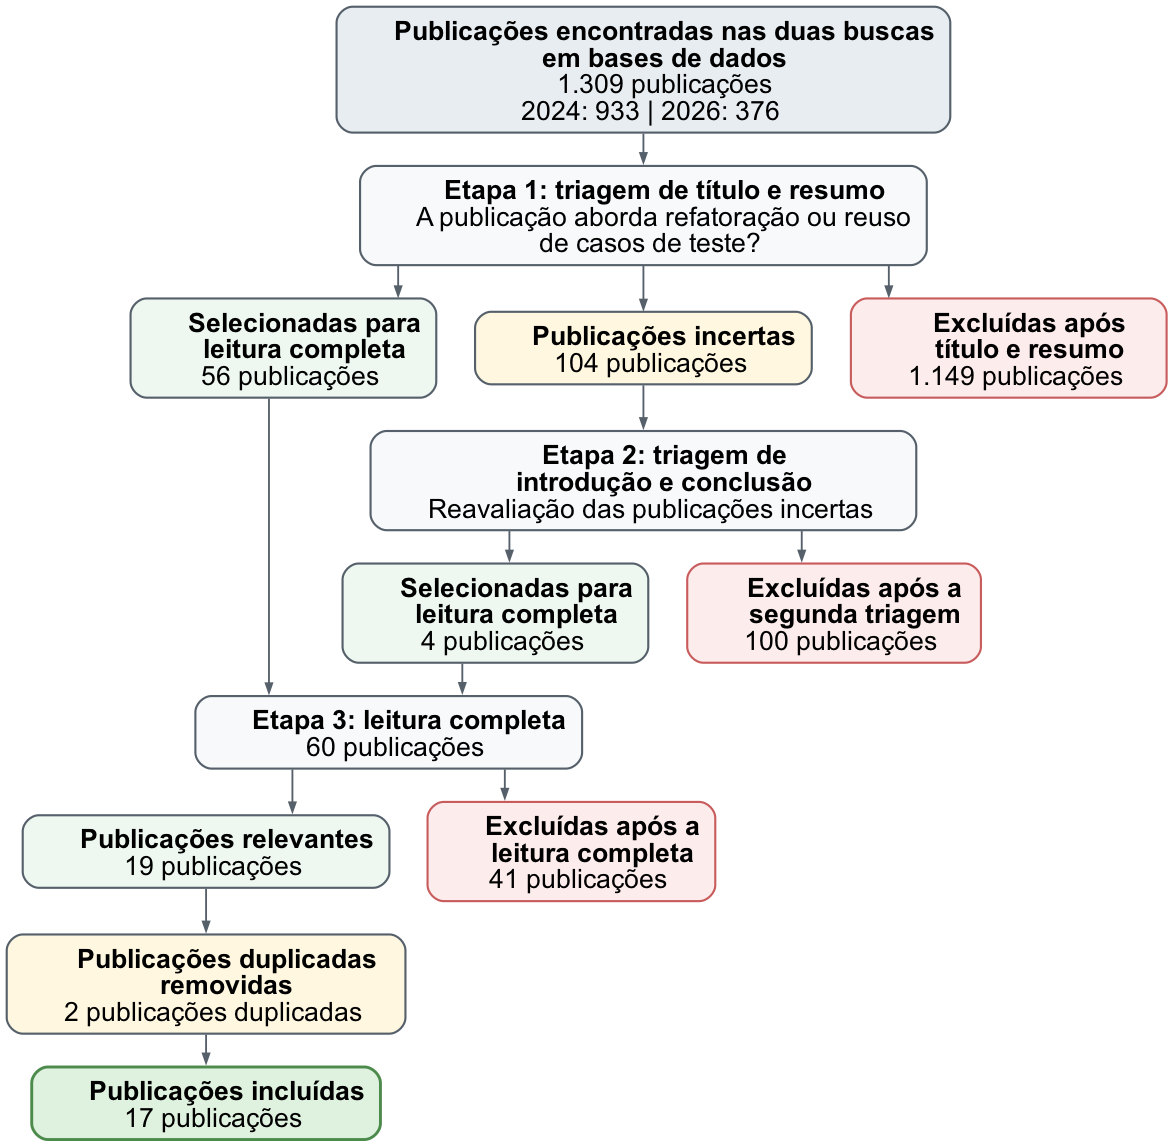
\includegraphics[width=\textwidth]{figures/systematic-study.png}
	\caption{Etapas consolidadas de filtragem das duas rodadas do estudo sistemático, das buscas iniciais até as 17 publicações incluídas}
	\label{figure:systematic-study}
	\fonte{Elaborado pelo autor.}
\end{figure}

Dos 19 registros que atenderam ao critério de inclusão, dois correspondiam a publicações recuperadas em mais de uma base de dados. Após a remoção dessas duplicatas, o estudo incluiu 17 publicações únicas. Os trabalhos selecionados mostram que a refatoração automática de testes está fragmentada entre objetivos e artefatos distintos. Alguns refatoram código de teste executável; outros, casos de teste em linguagem natural. Os objetivos também variam: substituição de \textit{mocks}, remoção de \textit{test smells}, melhoria de análise dinâmica ou reorganização de casos de teste. Essa diversidade confirma a relevância do tema, mas também indica que as abordagens existentes não oferecem uma arquitetura reusável para refatorar suítes completas com diferentes estratégias. Além disso, nenhuma delas trata a configuração implícita como um problema global sobre toda a suíte.

Três publicações relevantes pertencem ao mesmo grupo de autores \cite{wang:etal:2021,wang:etal:2022,wang:etal:2023}. Esses trabalhos examinam o uso de herança para criar \textit{mocks} de componentes que dependem de outros. Os autores argumentam que a herança não é o mecanismo mais adequado, pois introduz acoplamento com o código de aplicação. A proposta substitui automaticamente \textit{mocks} baseados em herança por \textit{mocks} de bibliotecas (e.g., Mockito\footnote{\url{https://site.mockito.org/}}). Em avaliação com projetos de código aberto, a abordagem identificou 334 candidatos e refatorou 276 (83\%). O foco, portanto, é substituir o mecanismo de \textit{mock}, e não reduzir a duplicação do código de teste.

\citeonline{pizzini:etal:2023:a} propõem a refatoração automática de \textit{eager test}. O principal desafio apontado é a detecção correta desse \textit{test smell}, pois um método do SUT pode aparecer na preparação do teste e não no exercício. Para reduzir falsos positivos, o teste só é classificado como afetado quando invocações ao SUT intercalam-se com asserções. Em 350 classes de teste, 312 apresentavam o \textit{test smell}; a abordagem refatorou 295 sem erros, e 17 falharam na execução. O tempo de execução aumentou 23\%. Uma limitação é a necessidade de reordenar os métodos refatorados para que não falhem, o que evita duplicação ao custo de violar a independência dos testes \cite{meszaros:2007}. Em trabalho subsequente, \citeonline{pizzini:etal:2023:b} apresentam o Sentinel, capaz de refatorar o \textit{eager test} e a duplicação de código. Dada uma classe, o Sentinel busca linhas comuns entre os métodos, agrupa os testes que as compartilham e os move para uma classe separada. A abordagem remove duplicação pela configuração implícita, porém opera sobre uma única classe.

\citeonline{santana:etal:2022} apresentam refatorações de \textit{assertion roulette} e \textit{duplicate assert}. No primeiro, a ferramenta indica os trechos e o usuário fornece uma descrição para cada asserção, em um processo semiautomático. No segundo, o método de teste é dividido automaticamente em dois ou mais métodos. A extração pode introduzir duplicação, pois o código compartilhado é replicado. Em experimento, a refatoração manual de \textit{assertion roulette} levou, em média, 78,30 segundos, contra 49,90 segundos com a ferramenta; para \textit{duplicate assert}, os tempos foram 107,20 e 2,55 segundos.

\citeonline{lambiase:etal:2020} apresentam o Dart, um plugin para o ambiente de desenvolvimento integrado (\textit{Integrated Development Environment} -- IDE) IntelliJ\footnote{\url{https://www.jetbrains.com/idea/}}, capaz de refatorar três \textit{test smells}: \textit{general fixture}, \textit{eager test} e \textit{lack of cohesion of test methods}. Diante de um \textit{general fixture}, o Dart extrai o teste para uma nova classe cujo método de configuração implícita contém apenas os acessórios necessários. Para o \textit{eager test}, decompõe o método de teste de modo que cada método resultante exercite um único método da classe de produção. Para a falta de coesão, agrupa e extrai métodos que cobrem as mesmas partes do código de aplicação. A detecção utiliza a ferramenta Taste, e o desenvolvedor decide se aplica a refatoração.

\citeonline{xuan:etal:2016} apresentam o B-Refactoring, voltado à análise dinâmica (i.e., à análise do programa enquanto os testes executam). A ferramenta reestrutura o código de teste para melhorar a eficácia do Nopol, que repara falhas no código de aplicação sob a condição de que cada caso de teste produza um único rastro de execução. O B-Refactoring divide um teste em fragmentos menores, cada um exercitando um caminho. A refatoração é sob demanda: o código original não é substituído de forma permanente. O foco, portanto, é melhorar a análise dinâmica, e não a manutenibilidade do código de teste.

\citeonline{shi:etal:2022} propõem um método de reuso orientado a agrupamento para casos de teste escritos em linguagem natural. Palavras-chave são extraídas, uma matriz de similaridade é construída e aplica-se o algoritmo \textit{spectral clustering} \cite{vonluxburg:2007}. O resultado são pacotes de casos de teste com alta similaridade semântica. A proposta não abrange o código de teste, apenas descrições em linguagem natural.

\citeonline{bernard:etal:2020} apresentam abordagem semelhante, na qual casos de teste em linguagem natural são agrupados pelo escopo funcional. A ferramenta Orbiter combina passos que representam a mesma ação com redações distintas e parametriza passos que diferem apenas em valores. Em experimento, o número total de passos reduziu-se em 18\%. Assim como \citeonline{shi:etal:2022}, o trabalho não refatora o código de teste, apenas os casos descritos em linguagem natural.

Por fim, \citeonline{hauptmann:etal:2015} examinam a refatoração de casos de teste em linguagem natural com técnicas de detecção de clones. Os casos são decompostos, trechos similares são extraídos e reusados, em comportamento análogo à configuração delegada. A abordagem é especialmente útil em testes de sistema (e.g., procedimentos comuns de autenticação em testes de aceitação). O processo é semiautomático: a ferramenta refatora as descrições em linguagem natural, mas o código de teste correspondente ainda precisa ser alterado manualmente.

\citeonline{gao:etal:2025} apresentam o UTRefactor, um \textit{framework} baseado em modelos de linguagem para refatorar automaticamente \textit{test smells} em testes unitários Java. A abordagem extrai contexto do código de teste e recorre a uma base externa com definições de \textit{test smells} e regras de refatoração descritas em uma linguagem específica de domínio. O modelo é guiado por encadeamento de raciocínio, com um mecanismo de verificação para tratar múltiplos \textit{test smells} no mesmo teste. Em 879 testes de seis projetos, o número de \textit{test smells} caiu de 2.375 para 265 (89\%). O UTRefactor superou a refatoração direta por modelo de linguagem em 61,82\% na eliminação de \textit{test smells} e também superou uma ferramenta baseada em regras. O foco, portanto, é remover \textit{test smells} no interior dos testes, e não redistribuir testes entre classes para aumentar o reuso da configuração implícita.

\citeonline{narang:etal:2025} apresentam a ferramenta \textit{Untangle to Weave} -- U2W, que detecta o \textit{test smell} DAT por análise de programa, separa o método em testes focados e, em seguida, combina testes estruturalmente semelhantes em testes unitários parametrizados. Em 42.334 testes de 49 projetos, o DAT apareceu em 95,9\% dos projetos, afetando em média 8,59\% dos testes. Foram refatorados 3.638 testes; a redução média de linhas executáveis nos testes afetados foi de 36,33\%. De 19 \textit{pull requests} submetidos, 16 foram aceitos. Assim como o UTRefactor, a U2W opera sobre o interior dos métodos de teste e sobre clones locais, sem tratar a configuração implícita da suíte como um todo.

\citeonline{derezinska:etal:2026} apresentam um plugin para o Eclipse, o TestSmellRefactorPlugin, voltado a programas Java com JUnit. O plugin detecta dez \textit{test smells} (e.g., roleta de asserções, asserção duplicada, teste ansioso e teste de número mágico) e refatora os testes por análise da AST. O desenvolvedor pode aceitar cada transformação ou aplicar, de uma vez, todas as ocorrências de um \textit{test smell} na classe. Em nove projetos, a detecção coincidiu em grande parte com a ferramenta tsDetect\footnote{\url{https://testsmells.org/}}, e os testes refatorados preservaram o resultado da execução. A abordagem é semiautomática e, como as anteriores, restringe-se a \textit{test smells} no interior da classe de teste.

\citeonline{guo:etal:2024} apresentam o PC-TRT, voltado ao reuso e à geração de casos de teste para cobertura de caminhos. A ferramenta compara caminhos da versão atual com caminhos cobertos por casos históricos: se a similaridade exceder um limiar, reusa-se o valor esperado do caso antigo; caso contrário, gera-se um caso novo por execução simbólica com o KLEE, ferramenta que explora caminhos do programa para gerar automaticamente entradas de teste. O objetivo é reduzir casos redundantes e preservar casos históricos de qualidade. O reuso, portanto, serve à cobertura estrutural, e não à manutenibilidade do código de teste.

\citeonline{wang:etal:2024} propõem o ATAG, que gera uma arquitetura de teste a partir dos fluxos de controle e de dados dos casos existentes, de modo a recuperar funções de teste coesas e pouco acopladas e, com isso, favorecer o reuso ao implementar novos casos. O FunBERT, baseado no \textit{Bidirectional Encoder Representations from Transformers} -- BERT, modelo de linguagem que representa o contexto das palavras nas duas direções da sentença, sugere nomes para essas funções. Em três conjuntos industriais, a arquitetura gerada melhorou, em média, o acoplamento em cerca de 26\% a 35\% e a coesão em cerca de 28\% a 50\% em relação ao desenho manual. O FunBERT obteve precisão de 97,9\%, revocação de 98,3\% e medida F1, média harmônica entre precisão e revocação, de 98,1\%. A proposta reorganiza funções de teste para reuso, mas não refatora a configuração implícita da suíte.

Por fim, \citeonline{almeida:etal:2026} combinam casos de teste sequenciais de funcionalidades individuais para gerar testes ainda sequenciais que exercitam funcionalidades concorrentes. A abordagem inclui análise de dependência entre passos e uma relação de conformidade que considera a ausência de saída observável. Quando o modelo de casos de uso não está disponível, os novos testes são obtidos pela permutação de passos (\textit{atoms}) dos casos existentes. Em avaliação com a Motorola Mobility, os testes gerados apresentaram cobertura e detecção de falhas superiores às da suíte produzida pelos engenheiros. O reuso, nesse caso, gera novos testes de concorrência a partir de testes já escritos, sem refatorar o código de teste em busca de manutenibilidade.

\subsection{Discussão}
\label{section:systematic-study-discussion}

As duas rodadas do estudo sistemático confirmam o quadro já esboçado na revisão exploratória. Há um conjunto diversificado de abordagens automáticas e semiautomáticas para refatorar ou reusar testes, porém nenhuma delas trata o problema que este trabalho formula. As técnicas encontradas operam sobre o interior de um método ou de uma classe, substituem mecanismos de \textit{mock}, removem \textit{test smells} pontuais, reorganizam descrições em linguagem natural ou reusam casos para cobertura e geração de novos testes. Mesmo quando extraem código comum para um método de configuração implícita, o recorte permanece local: o Sentinel restringe-se a uma única classe, e o Dart deixa ao desenvolvedor a decisão de aplicar a extração. Nenhuma abordagem redistribui os testes de uma suíte completa de modo a ampliar o reuso das sequências iniciais de configuração de acessórios.

Tampouco se identifica uma arquitetura reusável que separe as etapas de obtenção dos testes, medição de similaridade, agrupamento e refatoração, de forma que diferentes estratégias possam ser combinadas no mesmo fluxo. A similaridade, quando aparece, serve à redução de suíte, à priorização ou à recomendação de casos, e não à identificação de configurações de acessórios compartilhadas para reorganizar classes de teste.

Diante disso, a proposta deste trabalho é original em dois aspectos conjugados. Primeiro, trata a configuração implícita como um problema global de redistribuição de métodos entre classes de teste: métricas de similaridade e algoritmos de agrupamento são usados para considerar toda a suíte, de modo a reduzir a duplicação sem alterar o resultado observado dos testes. Segundo, materializa essa abordagem em uma arquitetura em \textit{pipeline} e no \textit{framework} Róża\footnote{\url{https://github.com/lucasPereira/roza}}, que instancia essa arquitetura com foco na estratégia de configuração implícita e admite a incorporação de outras estratégias. Nenhum dos trabalhos recuperados combina esses dois elementos.
